\section{Cenário Pessimista}

A Figura \ref{fig:cenario-pessimista} apresenta as receitas e custos acumulados no cenário pessimista considerando o projeto como um \gls{saas}. Nesse contexto, para o cálculo do acúmulo de receitas, estabeleceu-se um aumento mensal baixo de clientes tanto para o plano básico quanto para o profissional.

Os custos consideram somente os gastos com mão de obra, infraestrutura e mensalidades ou licenças das ferramentas utilizadas no desenvolvimento e manutenção da aplicação.

No cenário pessismista, o ponto de equilíbrio não é atingido no doze meses de análise e, ao fim desse intervalo de tempo, há um prejuízo de R\$ 337 mil.
\begin{figure}[h]
	\centering
	\caption{Cenário pessimista}
	\fbox{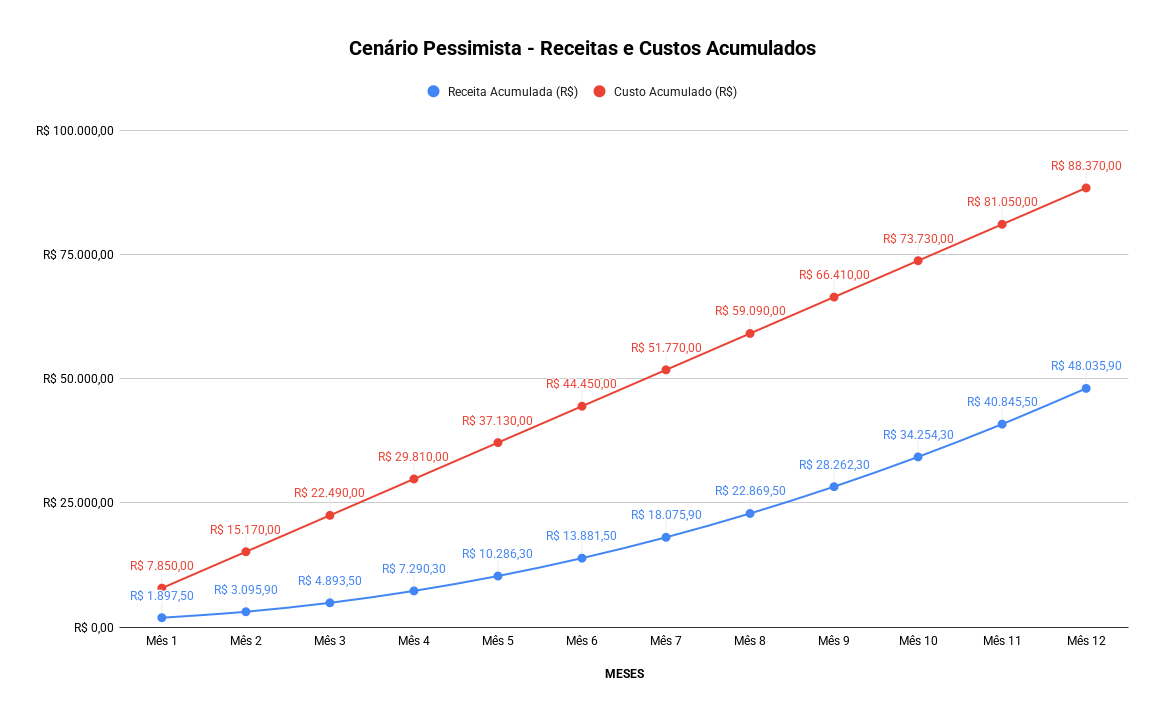
\includegraphics[width=0.9\textwidth]{cap05-viabilidade/imagens/cenario-pessimista.png}}
	\label{fig:cenario-pessimista}
	\fonte{Produzido pelos autores}
\end{figure}